%!TEX root = ../main.tex
%%%%%%%%%%%%%%%%%%%%%%%%%%%%%%%%%%
% Links:
%
% Difficulty: Companies: 
%%%%%%%%%%%%%%%%%%%%%%%%%%%%%%%%%%

\chapter{Median of two sorted arrays}
\label{ch:median_sorted_arrays}
\section*{Introduction}

The median is one of the most basic and important concept in statistics and probability theory and
it finds applications in almost every field of science. It is defined as the value that split a
certain data set into two equally sized halves: the higher and the lower half. For example the median of the
dataset $\{1,3,4,6,10,12,19\}$ is $6$ because we have $3$ elements greater and $3$ elements smaller
than $6$. When the size of the dataset is even, such element does not exists and thus the median is defined as the mean of the two middle elements;
For instance given the dataset $\{1,3,4,6,8,10,12,19\}$, the median is $\frac{6+8}{2}=7$.  

The problem covered in this chapter is about finding the median from a dataset provided as two
separate input list of values (you can imagine, for instance, that each of the input set comes from
a separate thread as part of a multithreaded application to analyze a large dataset).
Despite an obvious solution exists that pretty follows from the definition of
median, this problem is considered to be hard to solve optimally in a coding interview context
as it requires non-trivial insights and careful implementation.
But, despite its daunting reputation has been asked often during coding interviews.

For the rest of the chapter we will go throught the problem statement, and then we dive deeper into the
problem by discussing a number of possible approaches that will make us go from a naive and
inefficient to a more sophisticated but optimal solution. 

\section{Problem statement}
\begin{exercise}
You are given two \textbf{sorted} arrays $A$ and $B$ of size $m$ and $n$, respectively. Your task is
to write a function that takes as input $A$ and $B$ and returns the median of the two sorted arrays.
$A$ and $B$ con be considered to be proper subsets of a third dataset $C = A \cup B$. 

	\begin{example}
		\hfill \\
		Given two sorted arrays:
		\begin{itemize}
			\item $A=[1,4,6,10,15]$
			\item $B=[2,3,5,6]$
		\end{itemize}
		The median is $5$ (see Figure \ref{fig:median_sorted_arrays:example2}).
	\end{example}

	\begin{example}
		\hfill \\
		Given two sorted arrays:
		\begin{itemize}
			\item $A=[1,4,6,10]$
			\item $B=[2,3,5,6]$
		\end{itemize}
		The median is $\frac{5+4}{2} = 4.5$ (see Figure \ref{fig:median_sorted_arrays:example1}).
	\end{example}

\end{exercise}

\begin{figure}
	\label{fig:median_sorted_arrays:example2}
	\centering
	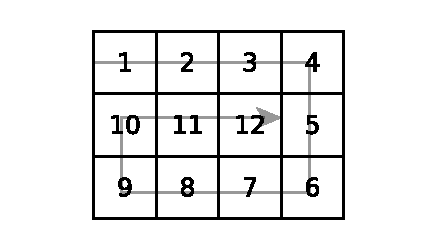
\includegraphics[scale=1.0]{sources/median_sorted_arrays/images/example2}
	\caption[Example of median of two sorted array.]{Example of median of two sorted array where the total number of elements is odd.}
\end{figure}

\begin{figure}
	\label{fig:median_sorted_arrays:example1}
	\centering
	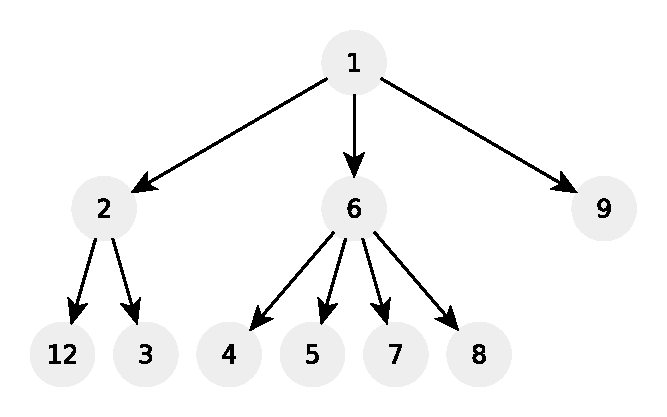
\includegraphics[scale=1.0]{sources/median_sorted_arrays/images/example1}
	\caption[Example of median of two sorted array.]{Example of median of two sorted array where the total number of element is even.}
\end{figure}


\section{Clarification Questions}

\begin{QandA}
	\item Can $A$ or $B$ be empty?
	\begin{answered}
		\textit{Yes, but you can assume that $|A \cup B| > 0$ i.e. at most one of the input array can be empty.}
	\end{answered}
	
\end{QandA}

\section{Discussion}
\label{median_sorted_arrays:sec:discussion}
Let's start our discussion by reviewing the concept of median. The median of a collection $C$ of $n$
elements is ($C_i$ represents the $i^{th}$ element of $C$):
\begin{itemize}
	\item $C_{\frac{n}{2}}$ if $n$ is odd (see Figure \ref{fig:median_sorted_arrays:example1})
	\item $\frac{C_{\floor{\frac{n}{2}}}+C_{\ceil{\frac{n}{2}}}}{2}$ if $n$ is even (see Figure
	\ref{fig:median_sorted_arrays:example2})
\end{itemize}
In simpler terms the median of a sorted collection is the element which divides the collections into
two equally sized halves, left and right, each with the same number of elements. 
If $n$ is even, clearly such element does not exists and thus the median is the defined to be the mean of the two middle
elements as shown in Figure \ref{fig:median_sorted_arrays:example1}.
Additionally, notice that because the collection is sorted then all the elements in the left half are smaller or equal then
the median and all the elements on the right half are larger. 

\subsection{Brute-force}
\label{median_sorted_arrays:sec:bruteforce}
Armed with the definition of median, we can immediately devise a simple and effective approach to
find it given the two input sorted arrays. The only difference between the problem statement and the
definition of median is that we are given two sorted arrays and not just one. Therefore it is
natural that the very first thing that should come to mind is to:
\begin{enumerate}
	\item create a third array $C = A \cup B$, which is the concatenation of the two input arrays
	\item proceed by sorting $C$,
	\item calculate the median (and not forgetting to take into consideration the parity of $|C|$)
\end{enumerate}

This approach is clearly correct as it is basically a direct consequence and application of the
definition of median given above, but it is far from being optimal, as we will see below. Listing
\ref{list:median_sorted_naive} shows a C++ implementation of this idea. Time and space complexities
of this approach are $O((n+m)log(n+m))$(because of sorting) and $O(s+m)$(space required by the third
array), respectively. Despite being suboptimal this solution has the benefit of being very short (only a few lines)
and easy to read, explain and understand.

\lstinputlisting[language=c++, caption={Naive implementation of solution to the problem of finding the median of two sorted arrays.},label=list:median_sorted_naive]{sources/median_sorted_arrays/median_sorted_arrays_solution1.cpp}


\subsection{Brute-force improved}
\label{median_sorted_arrays:sec:bruteforce_improved}
The brute-force approach can be improved a bit if we use the fact that the arrays are already
sorted. In the approach described in Section \ref{median_sorted_arrays:sec:bruteforce} we do not use
this fact and therefore we are forced to sort the entire array $C$ that we created by blindly juxtaposing $A$ and $B$ one after the other.
By taking advantage of the fact that the inputs are sorted we can create the array $C$ in a smarter way,
so that it is already sorted. In order to do so we will use the fact that you can merge two sorted array into a third sorted array in linear time.
You might be already familiar with this idea if you know how the famous merge-sort algorithm\cite{wiki:mergesort} works as the same operation is one of its two basic building blocks.
Listing \ref{list:median_sorted_naive_2} shows how this idea can be coded in C++. Notice how most of the code is now taken by the \inline{std::vector<T> mergeSortedArrays(const std::vector<T> &A,
const std::vector<T> &B)} function that 
is responsible for taking two sorted arrays (pay attention to the \inline{assert}) as input and returning a third sorted one. 

\lstinputlisting[language=c++, caption={Naive implementation of solution to the problem of finding the median of two sorted arrays using the merge part of merge-sort algorithm.},label=list:median_sorted_naive_2]{sources/median_sorted_arrays/median_sorted_arrays_solution2.cpp}

The time and complexities of this version are both $O(n+m)$, much better than the one from the solution presented in
Section \ref{median_sorted_arrays:sec:bruteforce} but, it is still suboptimal as this problem can be
solved in logarithmic time. We are going to see how in Section \ref{median_sorted_arrays:sec:log}.

\subsubsection{Merge sorted array in linear time}

\subsection{Logarithmic solution}
\label{median_sorted_arrays:sec:log}
Let's start by pointing out that the very essence of this problem is to try to figure out how the
merging the two arrays together into one would look like (like in the previous sections) but without
actually performing the merging itself.

The key ideas are:
\begin{itemize}
	\item we know exactly how big is the merged array ($C$)
	\item the left part of $C$, $C_l$ would be made up from portions of the smallest values of $A$
	and $B$. For instance, w.r.t. the example in Figure \ref{fig:median_sorted_arrays:example2} we
	can see that the left half (the first $5$ elements) of $A+B$ is made from the first two elements
	of $A$ and the smallest $3$ elements of $B$. Because $C$ will be sorted, only the smallest
	elements of $A$ and $B$ will contribute to its left half.
\end{itemize}

At the beginning we do not know exactly how many elements from $A$ will be part of the first half of
$C$, $C_l$. But we can try to search for this number. Let's suppose we try to construct $C_l$ by
using $i$ elements from $A$. Because we know the size of $C$ i.e. $s=n+m$ (the sum of the sizes of
$A$ and $B$), we also know the size of $C_l$, $s_2 = \frac{s}{2}$. Thus, we also know how many
elements we need to take from the left part of $B$ ($B_l$), i.e. $s_2 - i$.
